% !TeX encoding = UTF-8
% !TeX program = xelatex
% !BIB program = bibtex
% !TeX spellcheck = en_US

\documentclass{cjc}

\usepackage{booktabs}
\usepackage{algorithm}
\usepackage{algorithmic}
\usepackage{siunitx}
\usepackage{listings}
\usepackage{float}

\classsetup{
  % 配置里面不要出现空行
  title        = {浅谈区间操作及其数据结构},
  title*       = {Data structure for range operations},
  authors      = {
    author1 = {
      name         = {姜文渊},
      name*        = {JIANG Wen-yuan},
      affiliations = {aff1},
      biography    = {男,同济大学本科在读。},
      % 英文作者介绍内容包括:出生年, 学位(或目前学历), 职称, 主要研究领域(与中文作者介绍中的研究方向一致).
      biography*   = {Undergraduate student at Tongji University.},
      email        = {1951510@tongji.edu.cn},
      %phone-number = {0},  % 第1作者手机号码(投稿时必须提供,以便紧急联系,发表时会删除)
    },
  },
  % 论文定稿后,作者署名、单位无特殊情况不能变更。若变更,须提交签章申请,
  % 国家名为中国可以不写,省会城市不写省的名称,其他国家必须写国家名。
  affiliations = {
    aff1 = {
      name  = {同济大学\; 软件工程学院, 上海 中国\ 201804},
      name* = {School of Software Engineering, Tongji University, Shanghai, 201804, China},
    },
  },
  abstract     = {本文通过一个软件工程实践中的常见事例,对区间信息及区间操作进行了探究,进而引出了对支持高效区间操作的数据结构的需求。除了朴素的线性数据结构外,本文引入了几种支持区间操作的数据结构:前缀数组、ST表、树状数组、块状数组、线段树和Chtholly树;并分析了他们的实现、性能、应用场景及其局限性。这些数据结构各有特点:除了复杂度远好于朴素的结构外(一些文中的数据结构达到$O(log\,n)$),其实现与局限也各有不同。本文希望通过对这些数据结构进行比较,得出某些应用场景下的首选方案;本文也讨论了这些数据结构的后续发展,以期加深同学们对于数据结构的认识。
  },
  abstract*    = {This article uses a case in software engineering practice to explore range information and range operations, and then introduces the need for data structures that support efficient range operations. In addition to the simple linear data structure, this article introduces several data structures that support range operations: prefix array, ST table, BIT array, block array, segment tree and Chtholly tree; and analyzes their implementation, performance, application scenario and limitations. These data structures have their own features: in spite of the fact that the complexity of these structures is much better than the simple linear array (some can reach $O(log\,n)$), their implementation and limitations are also interesting. This article hopes to compare these data structures to get the preferred solution in certain application scenarios. This article also discusses the follow-up development of these data structures, in order to deepen students' understanding in data structures.},
  % 中文关键字与英文关键字对应且一致,应有5-7个关键词,不要用英文缩写
  keywords     = {数据结构,区间操作,线段树,前缀和,分块思想},
  keywords*    = {Data structure, Range operation, Segment tree, Prefix sum, Partition},
  %grants       = {
  %  本课题得到……基金中文完整名称(No.项目号)、
  %  ……基金中文完整名称(No.项目号)、
  %  ……基金中文完整名称(No.项目号)资助.
  %},
  % clc           = {TP393},
  doi           = {N/A},  % 投稿时不提供DOI号
  % received-date = {2019-08-10},  % 收稿日期
  % revised-date  = {2019-10-19},  % 最终修改稿收到日期,投稿时不填写此项
  % publish-date  = {2020-03-16},  % 出版日期
  % page          = 512,
}

\newcommand\dif{\mathop{}\!\mathrm{d}}

% hyperref 总是在导言区的最后加载
\usepackage{hyperref}

\lstset{basicstyle=\footnotesize\ttfamily,numberstyle=\tiny,numbers=none,frame=shadowbox,language=C++}

\begin{document}

\maketitle

\section{引言}

\subsection{本文的目的}

在诸多软件工程的实践中,我们会经常遇到对一个线性数据结构的诸多连续区间进行操作的需求。“线性数据结构”和“连续区间操作”的概念可能略显抽象,下面的例子可以让你对这些概念有一个感性的认识。

例如,在一个列车购票系统中,列车可以依次停靠多个站台,且列车上的总座位数$S$是有限的。我们将站台编号为$1..n$,在从站台$k-1$到站台$k$的列车上的已占用座位数为$s[k]$。则乘客购票时,会提供其上车的站台$i$和下车的站台$j$,则该购票系统需要查询在$[i,j)$这个区间中,列车上已经占用的座位数量的最大值,即$\max_{k\in(i,j]}s[k]$。若该值恰好等于总座位数$S$,则系统不能接受该乘客的购票请求;反之,我们则接受该乘客的购票请求,并将$(i,j]$这个区间中的所有$s[k]$都加上$1$。

在上面的例子中,“线性数据结构”是指记录被编号的站台间列车上占用座位人数的$s[k]$,而“查询$\max_{k\in(i,j]}s[k]$”和“把$(i,j]$这个区间中的所有$s[k]$都加上$1$”就是对于一个连续区间的操作。实际的生产需要中,将时间或者某个方向的空间抽象为线性结构,并对线性结构上的区间进行一系列操作,是十分常见的(尤其在计算机图形学等领域)。因而,研究支持快速进行区间操作的数据结构显得十分具有价值。

然而,笔者在诸多关于数据结构的各层次教材中(从写给小朋友的算法书,到各类本科生的课程教材),关于这类数据结构介绍甚少,因而在本文中,笔者将一些支持区间操作的数据结构进行了不系统的整理,并对其应用场景和性能进行了分析,供同学们参考学习。

\subsection{区间信息}

在一个线性数据结构$s[k],(k\in [0,n))$中,我们称$[i,j],([i,j]\subseteq [0,n))$为一个区间。自变量为区间的一个函数$f_s(i,j)$为区间信息。例如:
\begin{equation*}
  f_s(i,j) = \sum_{i\leq x \leq j}^{}s[x]
\end{equation*}
\begin{equation*}
  f_s(i,j) = \max_{i\leq x \leq j}s[x]
\end{equation*}
\begin{equation*}
  f_s(i,j) = \frac{1}{i-j+1}\sum_{i\leq x \leq j}^{}s[x]
\end{equation*}
\begin{equation*}
  f_s(i,j) = \text{Xor} _{i\leq x \leq j}s[x]
\end{equation*}
均是区间信息。注意到计算区间信息时$s$中的数据没有发生变化,但是我们也将查询区间信息视为一种区间操作。

\subsection{区间操作}

除了计算一些区间信息外,对$s$中某段区间所存数据的批量修改是最常见的一种区间操作。本文中区间操作有如下的形式:
\begin{equation*}
  \text{Op} _s(i,j,F(x))
\end{equation*}
其中,$F(x)$是对区间每一个元素的操作。例如,将$[i,j]$区间中的每一个数都加上$a$、将$[i,j]$区间中的每一个数都进行平方、将$[i,j]$区间中的每一个数都设为$b$等,都是典型的区间操作。

\subsection{区间操作的性质}
区间信息在很多时候可以认为是满足含幺半群的性质的信息。

常用的一些区间操作通常具有比较好的性质,可以用于简化问题的求解。其中,很多区间操作的性质可以和区间求和进行类比,我们记:
\begin{equation*}
  \text{sum\_range} _s(i,j) = \sum_{i\leq x \leq j}^{}s[x]
\end{equation*}
则不难证明,$\text{sum\_range} _s(i,j) = \text{sum\_range} _s(i,k) + \text{sum\_range} _s(k,j), k\in[i,j]$,即为区间的操作可以划分到子区间进行递归操作。求最大值、均值以及对区间进行加减乘除等赋值操作,均具有这样的性质。

另一种区间操作的性质被称为可重复贡献性质,这类性质是指对于区间信息的查询,有$x\, \text{opt}\, x = x$,即元素与自身做某个操作,仍然得到自身,例如$\max$和$\gcd$。而对于加和等操作,则没有这样的性质。

\subsection{一些约定}

本文为方便说明,仅考虑线性数据结构中的元素为正整数的情形。本文中的复杂度分析,均使用通常教材中的Big-O notation,即类似$O(n)$的表示方法。文中提供的代码片段的实现均使用C++或类似的伪代码写成,对于C++代码,遵循C++11标准。在复杂度的分析中,本着实用主义的理念,本文中将省略复杂度的证明。对于某些复杂度不十分显然的数据结构,本文采用事后测量的方式来验证理论所导出的复杂的的正确性,且主要考虑随机数据的情况。具体实现的程序见附录部分,且具体的测试数据见补充材料。

本文中有一些可能产生误解的名词,在这里约定其含义。

\paragraph{区间、区间信息和区间操作} 详见引言部分的说明。

\paragraph{在线算法和离线算法} 在计算机科学中,一个在线算法是指它可以以序列化的方式一个个的处理输入,也就是说在开始时并不需要已经知道所有的输入。相对的,对于一个离线算法,在开始时就需要知道问题的所有输入数据,而且在解决一个问题后就要立即输出结果。例如,选择排序在排序前就需要知道所有待排序元素,然而插入排序就不必。


\section{支持区间操作的数据结构}

下面我们将对一些常见的支持区间操作的数据结构进行分析。

\subsection{朴素的数组}

对于区间操作,一个最简单的想法就是按照其定义,对区间中的元素依次进行操作。例如,对于整数数组$s[n]$考虑以下几个操作:
\begin{enumerate}
  \item 求区间$[i,j]$的元素的和
  \item 求区间$[i,j]$的元素的最大值
  \item 将区间$[i,j]$中的每个元素都增加1
  \item 修改元素$s[i]$为$a$
\end{enumerate}
\subsubsection{实现方式}
利用数组存储这些元素,并用一个\lstinline{for}循环按照定义对每个元素进行计算即可,实现上十分简单且暴力。

\subsubsection{复杂度分析}
\paragraph{时间复杂度} 对于区间操作1、2、3,由于区间是随机给定的,故区间长度的期望正比于数组的大小,则每次操作的时间正比于区间长度,故对于每次操作,其复杂度为$O(n)$。而单点修改操作4,其复杂度仅为$O(1)$。
\paragraph{空间复杂度} 由于该数据结构没有引入额外的存储空间,因而其所占的内存为$O(n)$。
\subsubsection{适用范围与局限性}
由于没有引入任何优化,故该算法为在线算法,且支持几乎所有区间操作。
考虑m个请求,则处理所有这m个请求所需的时间复杂度为$O(mn)$,当$n$,$m$在同一个数量级时,其时间复杂度可视为$O(n^2)$,在数据量增大时,无疑是十分缓慢的。

\subsection{前缀数组}

如果我们只考虑对区间的查询操作,且查询操作具有类似加法一样可以差分的性质:
\begin{equation*}
  \text{sum\_range} _s(i,j) = \text{sum\_range} _s(k,j) - \text{sum\_range} _s(k,i)
\end{equation*}
\begin{equation*}
  k \leq i \leq j
\end{equation*}
我们则可以利用前缀数组进行高效的查询。公式里的求和与求差是抽象的,像求异或等操作,也具有类似的差分的性质。
\subsubsection{实现方式}
这里我们以查询区间$[i,j]$元素的和为例,另原数组为$s[n]$,引入前缀和数组$p[n]$,$p[n]$中元素$p[i]=s[0]+s[1]+s[2]+...+s[i]$。在实际实现中,使用$p[i]=p[i-1]+s[i]$,即可在一个\lstinline{for}循环中完成前缀数组的构建:
\begin{lstlisting}
p[0] = s[0];
for (int i = 1; i < n; i++)
{
    p[i] = p[i - 1] + s[i];
};
\end{lstlisting}
查询时,直接返回\lstinline{p[i]-p[j]+s[j]}即可。
\subsubsection{复杂度分析}
\paragraph{时间复杂度} 预处理时,构建前缀数组$p[n]$复杂度为$O(n)$。而区间查询操作,其复杂度仅为常数$O(1)$。如果对数据进行修改,则需重新建立前缀数组,复杂度为$O(n)$。
\paragraph{空间复杂度} 虽然该数据结构引入了额外的存储空间,但由于$p[n]$与$s[n]$大小同阶,故占用内存仍然为$O(n)$,只是常数略大。
\subsubsection{适用范围与局限性}
考虑m个请求,则处理所有这m个请求所需的时间复杂度为$O(m+n)$(包括预处理的时间),当$n$,$m$在同一个数量级时,其时间复杂度可视为$O(m)$,在数据量增大时,查询是十分快速的。

但该数据结构不支持对数据的高效修改,仅支持高效查询,属于离线的数据结构,且对于区间查询有差分性质的限制。

\subsection{ST表}
即使在不对区间进行修改的情况下,如果某种区间信息不具有差分的性质,也无法使用前缀数组进行高效的查询。ST表(Sparse Table,稀疏表)这类数据结构可以高效处理这类符合结合律且可重复贡献的区间信息查询问题。一种典型的这类问题被称为RMQ(Range Maximum/Minimum Query,区间最大/最小值查询)问题。
\subsubsection{实现方式}
以查询区间最大值为例,ST表使用一个二维数组$f(i,j)$存储区间区间$[i,i+2^j-1]$的最大值。

初始化时,首先有$f(i,0)=a_i$,其中$a_i$即是原数组中的$s[i]$。接下来利用动态规划的方式计算$f(i,j)$,由定义可知$f[i,j]=\max(f[i,j],f[i+2^{j-1},j])$。

查询时,对于每个询问的区间$[l,r]$,将其分为两个部分$[l,l+2^s-1]$与$[r-2^s+1,r]$,其中$s=\left \lfloor log_2 (r-l+1) \right \rfloor $通过查表可得$f[l,l+2^s-1]$与$f[r-2^s+1,r]$,则$max(f[l,l+2^s-1],f[r-2^s+1,r])$即为区间最大值。
\begin{figure}[htb]
  \centering
  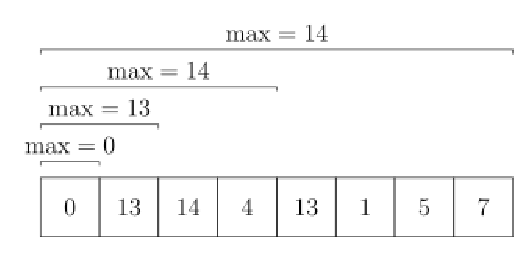
\includegraphics[width=\linewidth]{images/st.eps}
  \caption{ST表的示意图}
\end{figure}
\subsubsection{复杂度分析} 
\paragraph{时间复杂度} 对于预处理时$f[i,j]$的计算,计算的列数为$n$,而行数为$log_2\,n$,故其所耗时间为$O(n\, log \, n)$,而查询所用的时间为常数$O(1)$。
\paragraph{空间复杂度} 与$f[i,j]$所占空间一致,为$O(n\, log \, n)$。
\subsubsection{适用范围与局限性}

该数据结构不支持对数据的高效修改,仅支持高效查询(常数时间)。考虑m个请求,则处理所有这m个请求所需的时间复杂度为$O(m+n\, log \, n)$(包括预处理的时间),当$m$很大时,其时间复杂度可视为$O(m)$,应对大量查询是十分快速的。ST表属于离线的数据结构,且对于区间查询操作的信息需符合结合律且可重复贡献的性质。

\subsection{树状数组}
仍然考虑区间求和问题,为了克服前缀数组无法高效修改的局限性,我们引入了树状数组(Binary Index Tree, BIT),又称二进制下标树。
\subsubsection{实现方式}
朴素的数组的单点修改是$O(1)$,但是区间求和是$O(n)$。而前缀数组单点修改是$O(n)$,但是区间求和是$O(1)$。因此现在我们希望找到这样一种折中的方法:无论单点修改还是区间查询,它都能不那么慢地完成。

一个很自然的想法是,我们用一个数组$c$维护若干个小区间,单点修改时,只更新包含被修改元素的区间;在求区间和时,将$[0,i]$和$[0,j]$求出,用于前缀数组一样的方法计算$[i,j]$的和(差分即可)。极端情况下,如果$c$的每个元素对应一个元素,$c$就是朴素的数组;而如果$c$的每个元素对应$[0,i]$区间,$c$就是前缀数组。

一种分配$c$的方式巧妙地使用了数组下标的二进制表示形式。例如,当我们准备求前$11$项元素的和时,将$11$转化成二进制数$(1011)_2$,则可不断去掉二进制数最右边的一个1,从而得到三个区间:
\begin{equation*}
  (101\underline{0},101\underline{1}]
\end{equation*}
\begin{equation*}
  (10\underline{0}0,10\underline{1}0]
\end{equation*}
\begin{equation*}
  (\underline{0}000,\underline{1}000]
\end{equation*}
我们定义,二进制数最右边的一个1,连带着它之后的0为$\text{lowbit}(x)$。$\text{lowbit}(x)$可以使用位运算十分精巧地实现:
\begin{equation*}
  \text{lowbit}(x) = (x)\, \text{AND}\, (-x)
\end{equation*}
这里的$x$是补码表示的二进制数,读者可自行验证其正确性。这样,我们就可以让$c[i]$维护$s$的区间$(i-\text{lowbit}(i),i]$。查询前$i$项的和时,仅需将各个$(i-\text{lowbit}(i),i]$合并,如上面的三个区间所示,实现的代码片段如下:
\begin{lstlisting}
int c[MAXN];
......
int query(int n)
{
    int ans = 0;
    for (int pos = n; pos; pos -= lowbit(pos))
        ans += c[pos];
    return ans;
};
\end{lstlisting}
而更新时,则从含有$i$的区间$(i-\text{lowbit}(i),i]$开始,不断令$i=i+\text{lowbit}(i)$后再更新区间$(i-\text{lowbit}(i),i]$。一个更新的区间序列如下所示:
\begin{equation*}
  (\underline{100}100,\underline{100}110]
\end{equation*}
\begin{equation*}
  (\underline{10}0000,\underline{10}1000]
\end{equation*}
\begin{equation*}
  (\underline{1}00000,\underline{1}10000]
\end{equation*}
\begin{equation*}
  (000000,100000]
\end{equation*}
实现这一过程的代码片段为:
\begin{lstlisting}
void update(int i, int x)
{
    for (int pos = i; pos < MAXN; 
         pos += lowbit(pos))
        c[pos] += x;
};
\end{lstlisting}
区间查询时,只需和前缀数组类似,返回\lstinline{query(j) - query(i - 1)}即可。
\begin{figure}[htb]
  \centering
  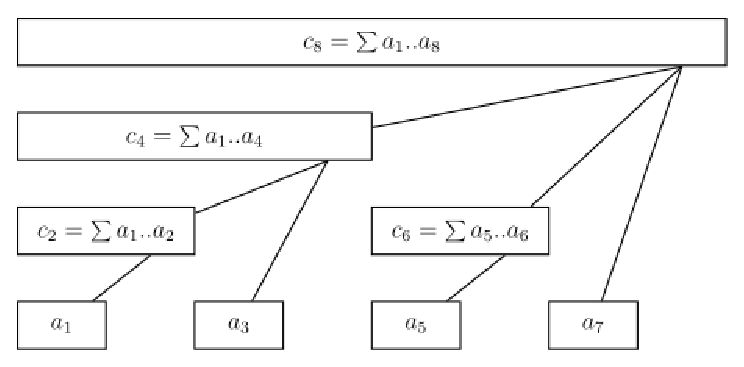
\includegraphics[width=\linewidth]{images/fenwick.eps}
  \caption{树状数组的示意图}
\end{figure}
\subsubsection{复杂度分析}
\paragraph{时间复杂度} 单点修改与区间查询的复杂度,由于二进制的性质,均为$O(log\,n)$,且由于位运算的使用,这个数据结构的常数较小。预处理相当于对每个元素进行一次更新,故为为$O(n\,log\,n)$
\paragraph{空间复杂度} 虽然该数据结构引入了额外的存储空间,但由于$c[n]$与$s[n]$大小同阶,故占用内存仍然为$O(n)$,只是常数略大。
\subsubsection{适用范围与局限性}
考虑m个请求,则处理所有这m个请求所需的时间复杂度为$O(m\,log\,n)$,当$n$,$m$在同一个数量级时,其时间复杂度可视为$O(n\,log\,n)$,远优于朴素的$O(n^2)$的数据结构。

但是对于区间修改的操作,树状数组的复杂度仍然不够理想。我们想要更进一步,实现对区间修改更加友好的数据结构。

\subsection{块状数组}
对于区间操作一种很直接的想法就是,把整体划分为若干个小块,对整块整体处理,零散块单独处理。块状数组就是利用分块思想处理区间操作的一种数据结构。这里我们考虑区间修改操作和区间求和操作。

\subsubsection{实现方式}
块状数组把一个长度为$n$的数组划分为$a$块,每块长度为$\frac{n}{a}$。对于一次区间操作,对区间內部的整块进行整体的操作,对区间边缘的零散块单独暴力处理。这里,块数既不能太少也不能太多。如果太少,区间中整块的数量会很少,我们要花费大量时间处理零散块;如果太多,又会让块的长度太短,失去整体处理的意义。

一般来说,我们取块数为$\sqrt{n}$,这在复杂度分析部分将进行详细的说明。

初始化块状数组时,要先划定出每个块所占据的范围:
\begin{lstlisting}
int sq = sqrt(n);
for (int i = 1; i <= sq; ++i)
{
    st[i] = n / sq * (i - 1) + 1;
     // st[i]表示i号块的第一个元素的下标
    ed[i] = n / sq * i;
     // ed[i]表示i号块的最后一个元素的下标
};
ed[sq] = n;
 //剩余的元素纳入最后一块中
for (int i = 1; i <= sq; ++i)
    size[i] = ed[i] - st[i] + 1;
 // 预处理每个块的大小
\end{lstlisting}
之后,对每个元素确定其所属的分块:
\begin{lstlisting}
for (int i = 1; i <= sq; ++i)
    for (int j = st[i]; j <= ed[i]; ++j)
        bel[j] = i; // 表示j号元素归属于i块
\end{lstlisting}
然后就可以读入数据,并对数据进行预处理:
\begin{lstlisting}
for (int i = 1; i <= n; ++i)
    A[i] = read(); // A[i]为原始数据
for (int i = 1; i <= sq; ++i)
    for (int j = st[i]; j <= ed[i]; ++j)
        sum[i] += A[j];
        // sum[i]保存第i个块的和
\end{lstlisting}
 
\paragraph{进行区间修改时} 当$x$与$y$在同一块内时,直接暴力修改原数组和\lstinline{sum}数组:
\begin{lstlisting}
if (bel[x] == bel[y])
    for (int i = x; i <= y; ++i)
    {
        A[i] += k;
        sum[bel[i]] += k;
    };
\end{lstlisting}
否则,先暴力修改左右两边的零散区间,然后对中间的整块打上标记:
\begin{lstlisting}
for (int i = x; i <= ed[bel[x]]; ++i)
{
    A[i] += k;
    sum[bel[i]] += k;
};
for (int i = st[bel[y]]; i <= y; ++i)
{
    A[i] += k;
    sum[bel[i]] += k;
};
for (int i = bel[x] + 1; i < bel[y]; ++i)
    mark[i] += k;
\end{lstlisting}

\paragraph{进行区间查询时} 如果左右两边在同一块,直接暴力计算区间和:
\begin{lstlisting}
if (bel[x] == bel[y])
    for (int i = x; i <= y; ++i)
        s += A[i] + mark[bel[i]]; 
        // 注意要加上标记
\end{lstlisting}
否则,暴力计算零碎块,再处理整块:
\begin{lstlisting}
for (int i = x; i <= ed[bel[x]]; ++i)
    s += A[i] + mark[bel[i]];
for (int i = st[bel[y]]; i <= y; ++i)
    s += A[i] + mark[bel[i]];
for (int i = bel[x] + 1; i < bel[y]; ++i)
    s += sum[i] + mark[i] * size[i]; 
    // 注意标记要乘上块的长度
\end{lstlisting}

\subsubsection{复杂度分析}
\paragraph{时间复杂度} 在最坏情况下,我们要处理接近个$\sqrt{n}$整块,还要对长度为$\frac{2n}{\sqrt{n}}$的零散块单独处理,故时间复杂度为$O(\sqrt{n})$。
\paragraph{空间复杂度} 虽然该数据结构引入了额外的存储空间,但由于$sum$等数组比$A$小($O(\sqrt{n})$),故占用内存仍然为$O(n)$,只是常数略大。
\subsubsection{适用范围与局限性}
分块的时间复杂度比不上树状数组这些对数级算法,但其可以支持的操作无需满足一些特殊的性质(比如结合律等),因而对于某些树状数组和后面的各种算法都无法支持的特殊的区间操作,使用块状数组是性能较好的选择。

\subsection{线段树}

如果从树的角度来观察分块数组,不难发现,其实分块数组是一种具有三层的多叉树。人们进一步考虑到,由于一些区间操作具有结合律,故而可以将区间二分,对左右两部分分别递归地求解,最后得到所需的答案。将一个长度不为1的区间分为两个子区间,作为树的节点保存起来,这样的数据结构被称为线段树。后续人们又向线段树中加入了延迟求值的机制(即通常所说的懒标记),使得其对区间操作的复杂度又得到了优化。

\subsubsection{实现方式}
这里以求区间的和为例进行说明。

设线段树的根节点编号为$1$,用数组$d$来保存我们的线段树,$d[i]$用来保存线段树上编号为$i$的节点的值(这里每个节点所维护的值就是这个节点所表示的区间总和)。由于这里采用堆的存储方式,故不难得到,$d[i]$的左孩子是$d[i*2]$,$d[i]$的右孩子是$d[i*2+1]$。若$d[i]$维护的区间是$[s,t]$,则其左孩子维护的区间是$[s,\frac{s+t}{2}]$,其右孩子维护的区间是$[\frac{s+t}{2}+1,t]$。建立线段树的过程可以利用递归进行:
\begin{lstlisting}
void build(int s, int t, int p) {
  // 对 [s,t] 区间建立线段树,当前根的编号为 p
  if (s == t) {
    d[p] = a[s];
    return;
  }
  int m = s + ((t - s) >> 1);
  // 移位运算符的优先级小于加减法,所以加上括号
  // 如果写成 (s + t) >> 1 可能会超出 int 范围
  build(s, m, p * 2), build(m + 1, t, p * 2 + 1);
  // 递归对左右区间建树
  d[p] = d[p * 2] + d[(p * 2) + 1];
}
\end{lstlisting}

查询时,亦可利用线段树的递归特性,拆分区间进行查询:
\begin{lstlisting}
int getsum(int l, int r, int s, int t, int p) {
// [l, r] 为查询区间, 
// [s, t] 为当前节点包含的区间, 
// p 为当前节点的编号
  if (l <= s && t <= r)
    return d[p];  
// 当前区间为询问区间的子集时直接返回当前区间的和
  int m = s + ((t - s) >> 1), sum = 0;
  if (l <= m) sum += getsum(l, r, s, m, p * 2);
  // [l, m] 与询问区间有交集,
  // 则递归查询左儿子
  if (r > m) sum += 
   getsum(l, r, m + 1, t, p * 2 + 1);
  // [m + 1, r] 与询问区间有交集,
  // 则递归查询右儿子
  return sum;
}
\end{lstlisting}

在修改区间时,为了避免对区间的每一个元素进行修改,我们引入“懒标记”的机制,延后对于节点的修改。每次执行修改时,我们通过打标记的方法表明该节点对应的区间在某一次操作中被更改,但不更新该节点的子节点的信息。实质性的修改则在下一次访问带有标记的节点时才进行。例如,对区间上的每个元素都加上某个值:
\begin{lstlisting}
void update(int l, int r, 
            int c, 
            int s, int t, 
            int p) {
// [l, r] 为修改区间, 
// c 为被修改的元素的变化量, 
// [s, t] 为当前节点包含的区间, 
 // p 为当前节点的编号
  if (l <= s && t <= r) {
    d[p] += (t - s + 1) * c, b[p] += c;
    return;
  }  
// 当前区间为修改区间的子集时
// 直接修改当前节点的值,
// 然后打标记,结束修改
  int m = s + ((t - s) >> 1);
  if (b[p] && s != t) {
// 如果当前节点的懒标记非空,
// 则更新当前节点两个子节点的值和懒标记值
    d[p * 2] += b[p] * (m - s + 1);
    d[p * 2 + 1] += b[p] * (t - m);
    b[p * 2] += b[p];
    b[p * 2 + 1] += b[p];  
    // 将标记下传给子节点
    b[p] = 0;                                
    // 清空当前节点的标记
  }
  if (l <= m) 
   update(l, r, c, s, m, p * 2);
  if (r > m) 
   update(l, r, c, m + 1, t, p * 2 + 1);
  d[p] = d[p * 2] + d[p * 2 + 1];
}
\end{lstlisting}

对于引入了懒标记的线段树,查询函数也应当进行相应的修改:
\begin{lstlisting}
int getsum(int l, int r, int s, int t, int p) {
  // [l, r] 为查询区间, 
  // [s, t] 为当前节点包含的区间, 
  // p 为当前节点的编号
  if (l <= s && t <= r) return d[p];
  // 当前区间为询问区间的子集时
  // 直接返回当前区间的和
  int m = s + ((t - s) >> 1);
  if (b[p]) {
    // 如果当前节点的懒标记非空,
    // 则更新当前节点两个子节点的值和懒标记值
    d[p * 2] += b[p] * (m - s + 1);
    d[p * 2 + 1] += b[p] * (t - m);
    b[p * 2] += b[p];
    b[p * 2 + 1] += b[p];  
    // 将标记下传给子节点
    b[p] = 0;                                    
    // 清空当前节点的标记
  }
  int sum = 0;
  if (l <= m) 
    sum = getsum(l, r, s, m, p * 2);
  if (r > m)
    sum += getsum(l, r, m + 1, t, p * 2 + 1);
  return sum;
}
\end{lstlisting}

\subsubsection{复杂度分析}
\paragraph{时间复杂度} 不难发现,线段树的深度是$\left \lceil log_2\,n \right \rceil $的,故其各个操作的时间复杂度为$O(log\,n)$。% ,但在极端情况下,可能退化至$O(n)$。
\paragraph{空间复杂度} 使用堆式存储时,一般为保险起见,$d$的大小设为$4n$,故占用内存仍然为$O(n)$,只是常数略大。
\subsubsection{适用范围与局限性}
线段树是较为通用的,且较快的支持区间操作的数据结构,除了其实现较为繁杂(尤其当涉及懒标记和多个操作时),基本上满足了常规使用的需求。

对于线段树的修改与查询都是在线的,且复杂度都能够接受,故线段树在生产实践中得到了广泛的使用。

\subsection{Chtholly树}

虽然线段树在理论上解决了绝大部分的区间操作问题,但对于复杂的功能(例如求区间第k大值,求区间元素n次方和),线段树的实现方式过于复杂,代码量较大,对于代码的维护比较不友好。出于实践上的需求,加上大部分情况下,区间操作时较为随机的,人们又构建了一种实现简单,且随机情况下性能极佳的,基于红黑树的数据结构:Chtholly树。

\subsubsection{实现方式}
Chtholly树的思想在于随机数据下的区间赋值操作很可能让大量元素变为同一个数。所以我们以三元组\lstinline{<l,r,v>}的形式保存数据(意为区间$[l,r]$中的元素的值都是$v$):
\begin{lstlisting}
# define ll long long
......
struct node
{
    ll l, r;
    mutable ll v; //这里mutable保证v可被操作
    node(ll l, ll r, ll v) : l(l), r(r), v(v) {} 
    bool operator<(const node &o) const 
    { return l < o.l; };
    //重载小于运算符,供std::set使用
};
\end{lstlisting}
这样的节点存储到\lstinline{std::set}里,就完成了Chtholly树的建立,代码量十分简短。
\begin{lstlisting}
set<node> tree;
\end{lstlisting}
进行区间操作时并不总是那么幸运,原本连续的区间可能会被断开。我们需要一个函数来实现“断开”的操作,把\lstinline{<l,r,v>}断成\lstinline{<l,pos-1,v>}和\lstinline{<pos,r,v>}:
\begin{lstlisting}
set<node>::iterator split(ll pos)
{
    auto it = tree.lower_bound(node(pos, 0, 0)); 
    // 寻找左端点大于等于pos的第一个节点
    if (it != tree.end() && it->l == pos) 
    // 如果已经存在以pos为左端点的节点,直接返回
        return it;
    it--; // 否则往前数一个节点
    ll l = it->l, r = it->r, v = it->v;
    tree.erase(it); // 删除该节点
    tree.insert(node(l, pos - 1, v)); 
    // 插入<l,pos-1,v>和<pos,r,v>
    return tree.insert(node(pos, r, v)).first; 
    // 返回以pos开头的那个节点的迭代器
    // insert默认返回值是一个pair,
    // 第一个成员是我们要的
};
\end{lstlisting}
之后,对于一些复杂的操作,我们从\lstinline{std::set}里用\lstinline{split}取出相应的元素,然后使用朴素且暴力的方法操作即可。例如,区间赋值操作:
\begin{lstlisting}
void assign(ll l, ll r, ll v)
{
    auto end = split(r + 1);
    auto begin = split(l); 
    // 顺序不能颠倒
    tree.erase(begin, end); 
    // 清除一系列节点
    tree.insert(node(l, r, v)); 
    // 插入新的节点
};
\end{lstlisting}
又如,区间元素同时加上一个数,直接取出后依次相加即可:
\begin{lstlisting}
void add(ll l, ll r, ll v)
{
    auto end = split(r + 1);
    for (auto it = split(l); it != end; it++)
        it->v += v;
};
\end{lstlisting}
求第k大值时,直接取出后用\lstinline{std::sort}排序即可:
\begin{lstlisting}
ll kth(ll l, ll r, ll k)
{
    auto end = split(r + 1);
    vector<pair<ll, ll>> v; 
    // 这个pair里存节点的值和区间长度
    for (auto it = split(l); it != end; it++)
        v.push_back(
        make_pair(it->v, it->r - it->l + 1));
    sort(v.begin(), v.end()); 
    // 直接按节点的值的大小排下序
    for (int i = 0; i < v.size(); i++) 
    // 然后挨个丢出来,直到丢出k个元素为止
    {
        k -= v[i].second;
        if (k <= 0)
            return v[i].first;
    };
};
\end{lstlisting}
查询n次方和亦然:
\begin{lstlisting}
ll sum_of_pow(ll l, ll r, ll x, ll y)
{
    ll tot = 0;
    auto end = split(r + 1);
    for (auto it = split(l); it != end; it++)
        tot = (tot + qpow(it->v, x, y) 
        * (it->r - it->l + 1)) % y; 
        // qpow为快速幂
    return tot;
};
\end{lstlisting}

\subsubsection{复杂度分析}
\paragraph{时间复杂度} 在随机数据的情况下Chtholly树的复杂度为$O(n\,log\,log\,n)$。具体的证明较为复杂,笔者在这里就不再赘述了。
\paragraph{空间复杂度} 由于该数据结构依托于\lstinline{std::set},因而其所占的内存为$O(n)$。
\subsubsection{适用范围与局限性}
Chtholly树的实现中,绝大部分进行实际计算的操作都是朴素的暴力求解,故而对于各类复杂的区间操作,Chtholly树都能胜任。但是,如果输入的数据具有严重的偏向性,不能保证随机性,则Chtholly树的复杂度将会逐渐接近朴素的数组实现。

\section{各数据结构实际测评}

在本部分中,我们首先比较各类数据结构在随机查询任务下的性能;接着,对于可以在线操作的数据结构,我们比较其在特定随机任务下的性能。测试的环境为常见的x86兼容机,操作系统与编译器等具体信息见附录部分。

\subsection{区间求和查询的性能比较}

\paragraph{参与比较的算法}朴素的数组,前缀数组,树状数组,块状数组,线段树。
\paragraph{输入格式} 第一行为两个整数$N$和$M$,表示初值为$N$个整数,供有$M$条询问,接下来$N$行,每行一个整数表示初值,接下来$M$行,每行两个整数$l$和$r$,表示查询的区间。保证$0\leq l \leq r \leq N$。

在不同的$N$下,令$M=10000$为固定值,考察程序运行的相对时间,如下图所示:
\begin{figure}[H]
  \centering
  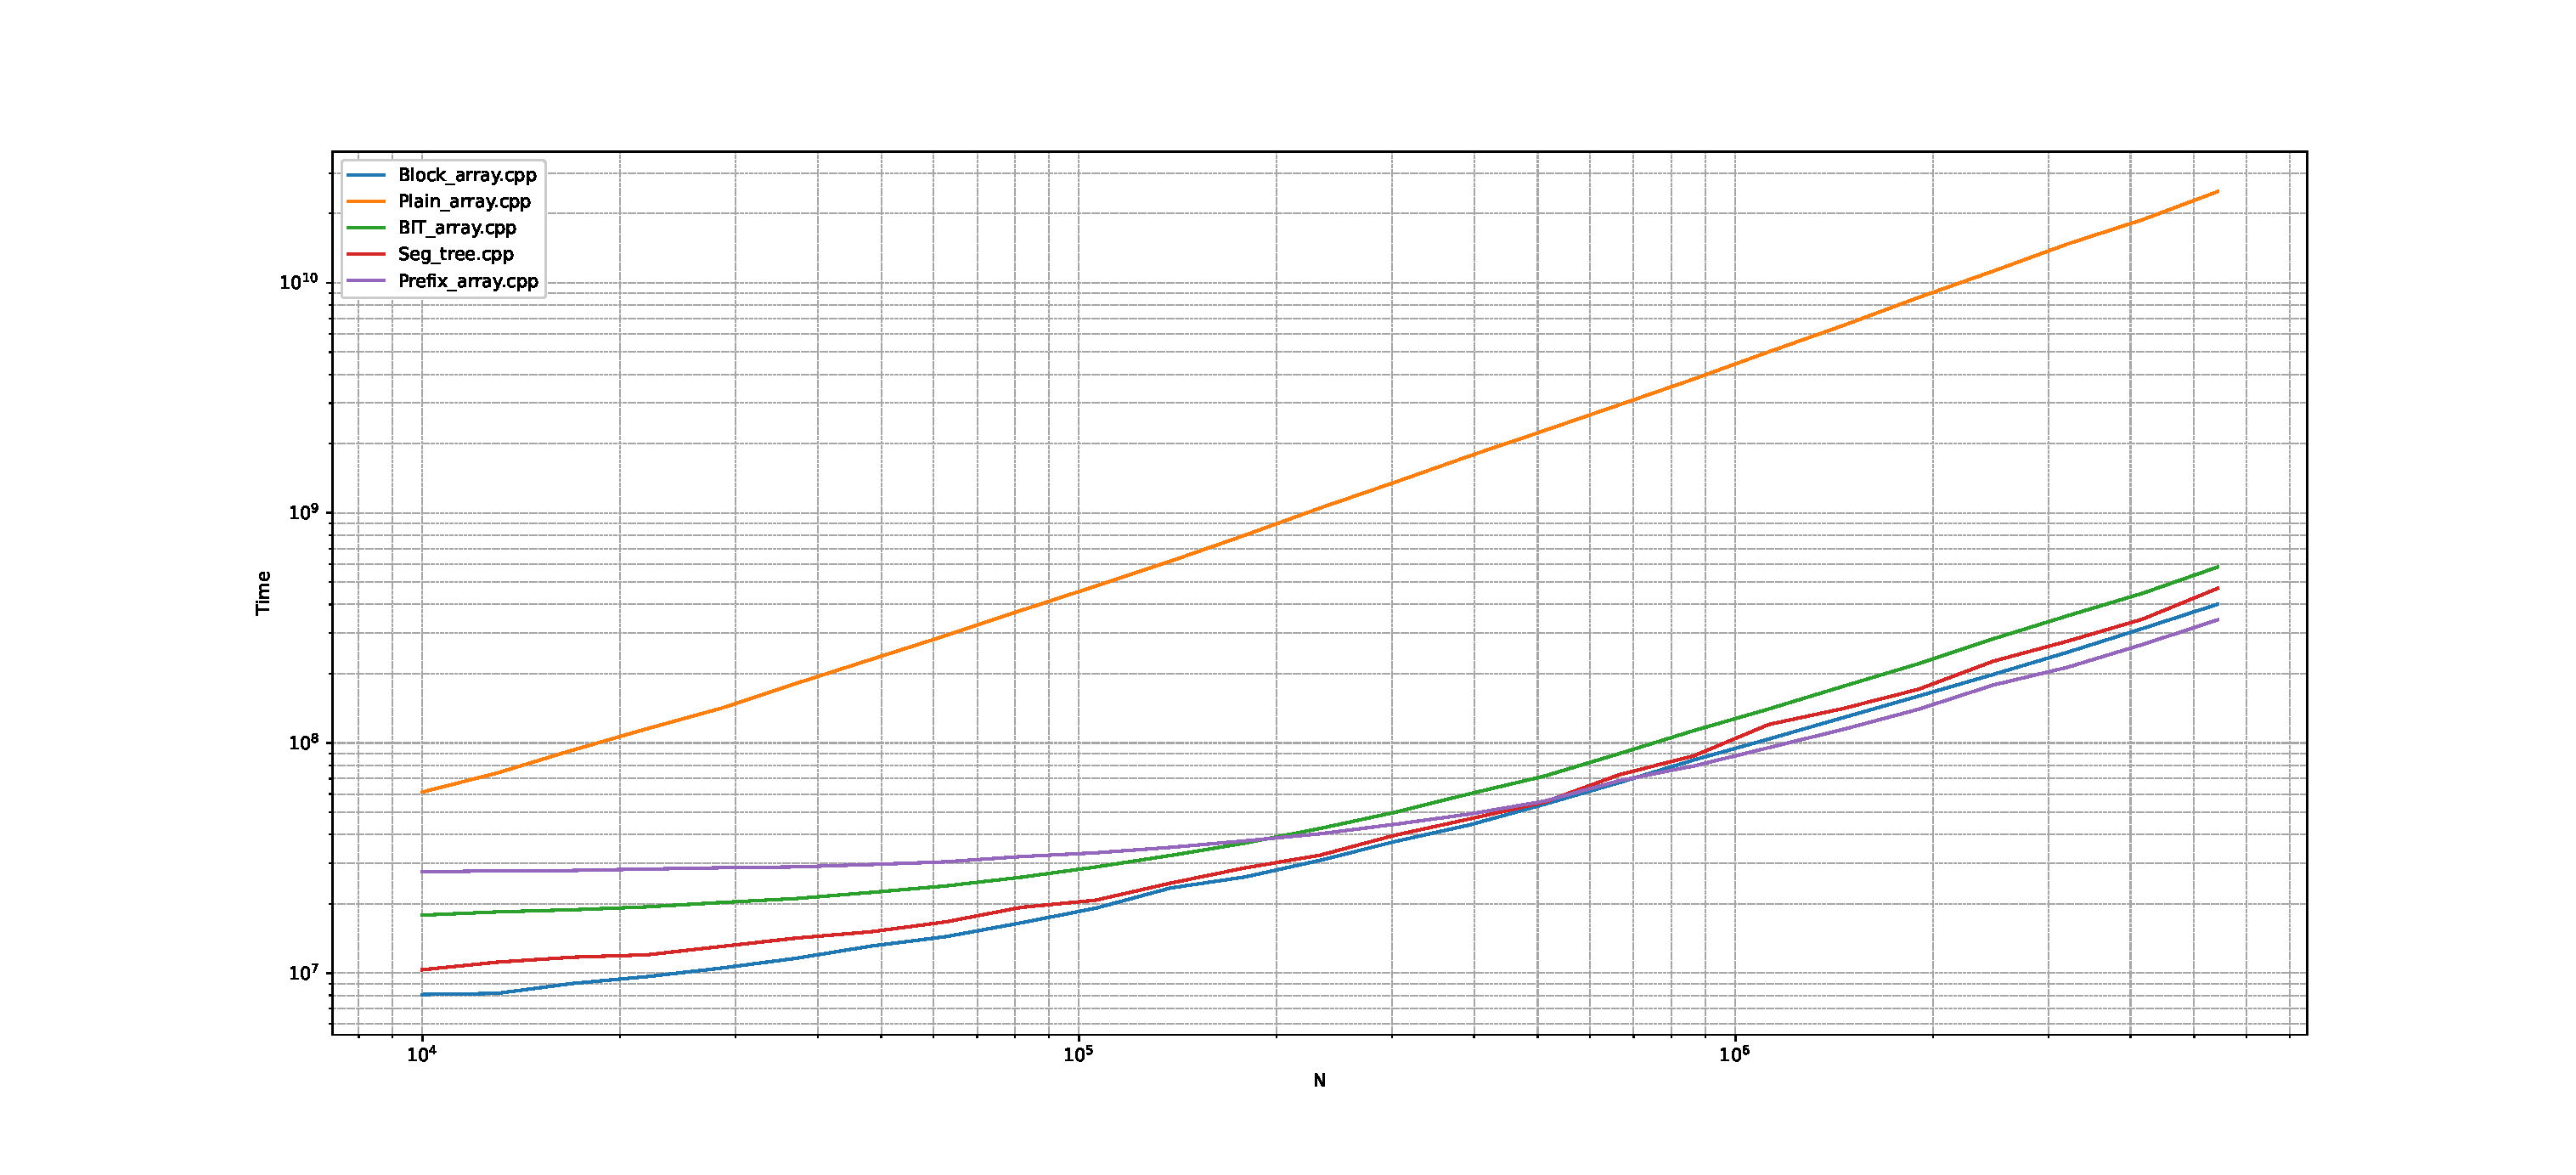
\includegraphics[width=\linewidth]{images/performance1.eps}
  \caption{查询任务下各数据结构的性能(双对数图,$M$固定)}
\end{figure}
由上图可见,除了朴素实现外,其余数据结构都有较好的时间复杂度。而且由于数据的随机性,使得分块等非对数复杂度的算法实际上也获得了与对数复杂度算法相似的性能。

在不同的$N$下,令$M=N$,考察程序运行的相对时间,如下图所示:
\begin{figure}[H]
  \centering
  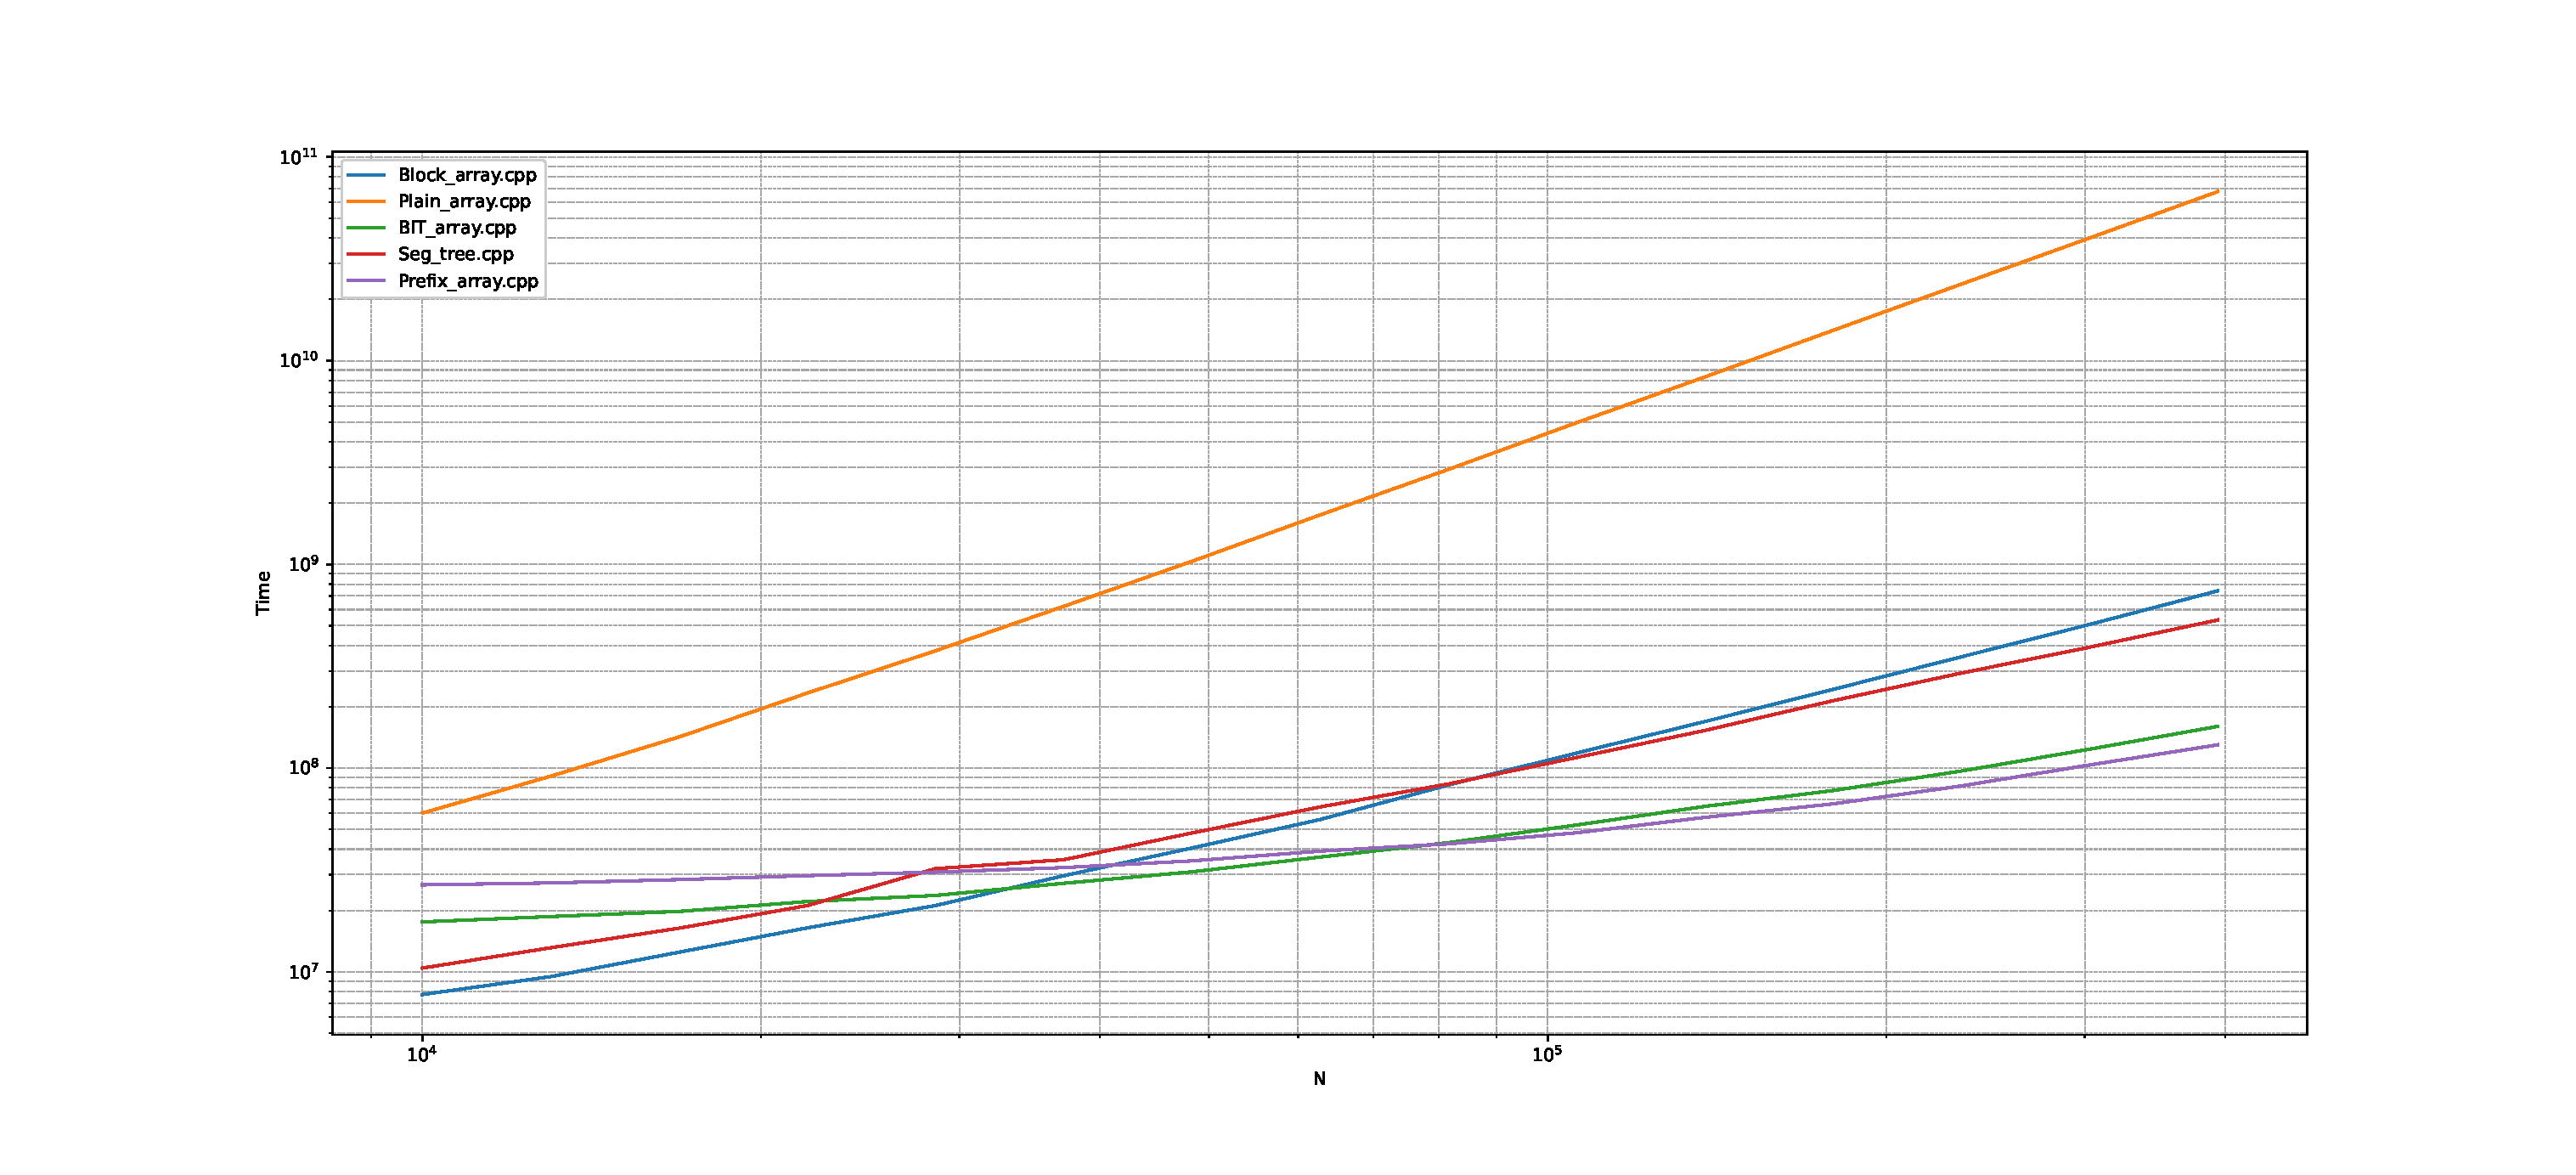
\includegraphics[width=\linewidth]{images/performance2.eps}
  \caption{查询任务下各数据结构的性能(双对数图,$M=N$)}
\end{figure}
由上图可见,当$M$与$N$同阶时,各数据结构的复杂度和理论计算相符。此时,分块等非对数复杂度的算法与对数复杂度的算法有来显著差距。

\subsection{区间加法与区间求最值查询的性能比较}
\paragraph{参与比较的算法} 线段树,Chtholly树。
\paragraph{输入格式} 第一行为两个整数$N$和$M$,表示初值为$N$个整数,供有$M$条询问,接下来$N$行,每行一个整数表示初值,接下来$M$行,每行四个整数$\text{op}$、$l$、$r$和$v$,。$\text{op}=1$时,表示查询区间$[l,r]$上的最大值;$\text{op}=2$时,表示区间$[l,r]$上所有元素都赋值为$v$,区间加上保证$0\leq l \leq r \leq N$。

在不同的$N$下,令$M$与$N$相同,考察程序运行的相对时间,如下图所示:
\begin{figure}[H]
  \centering
  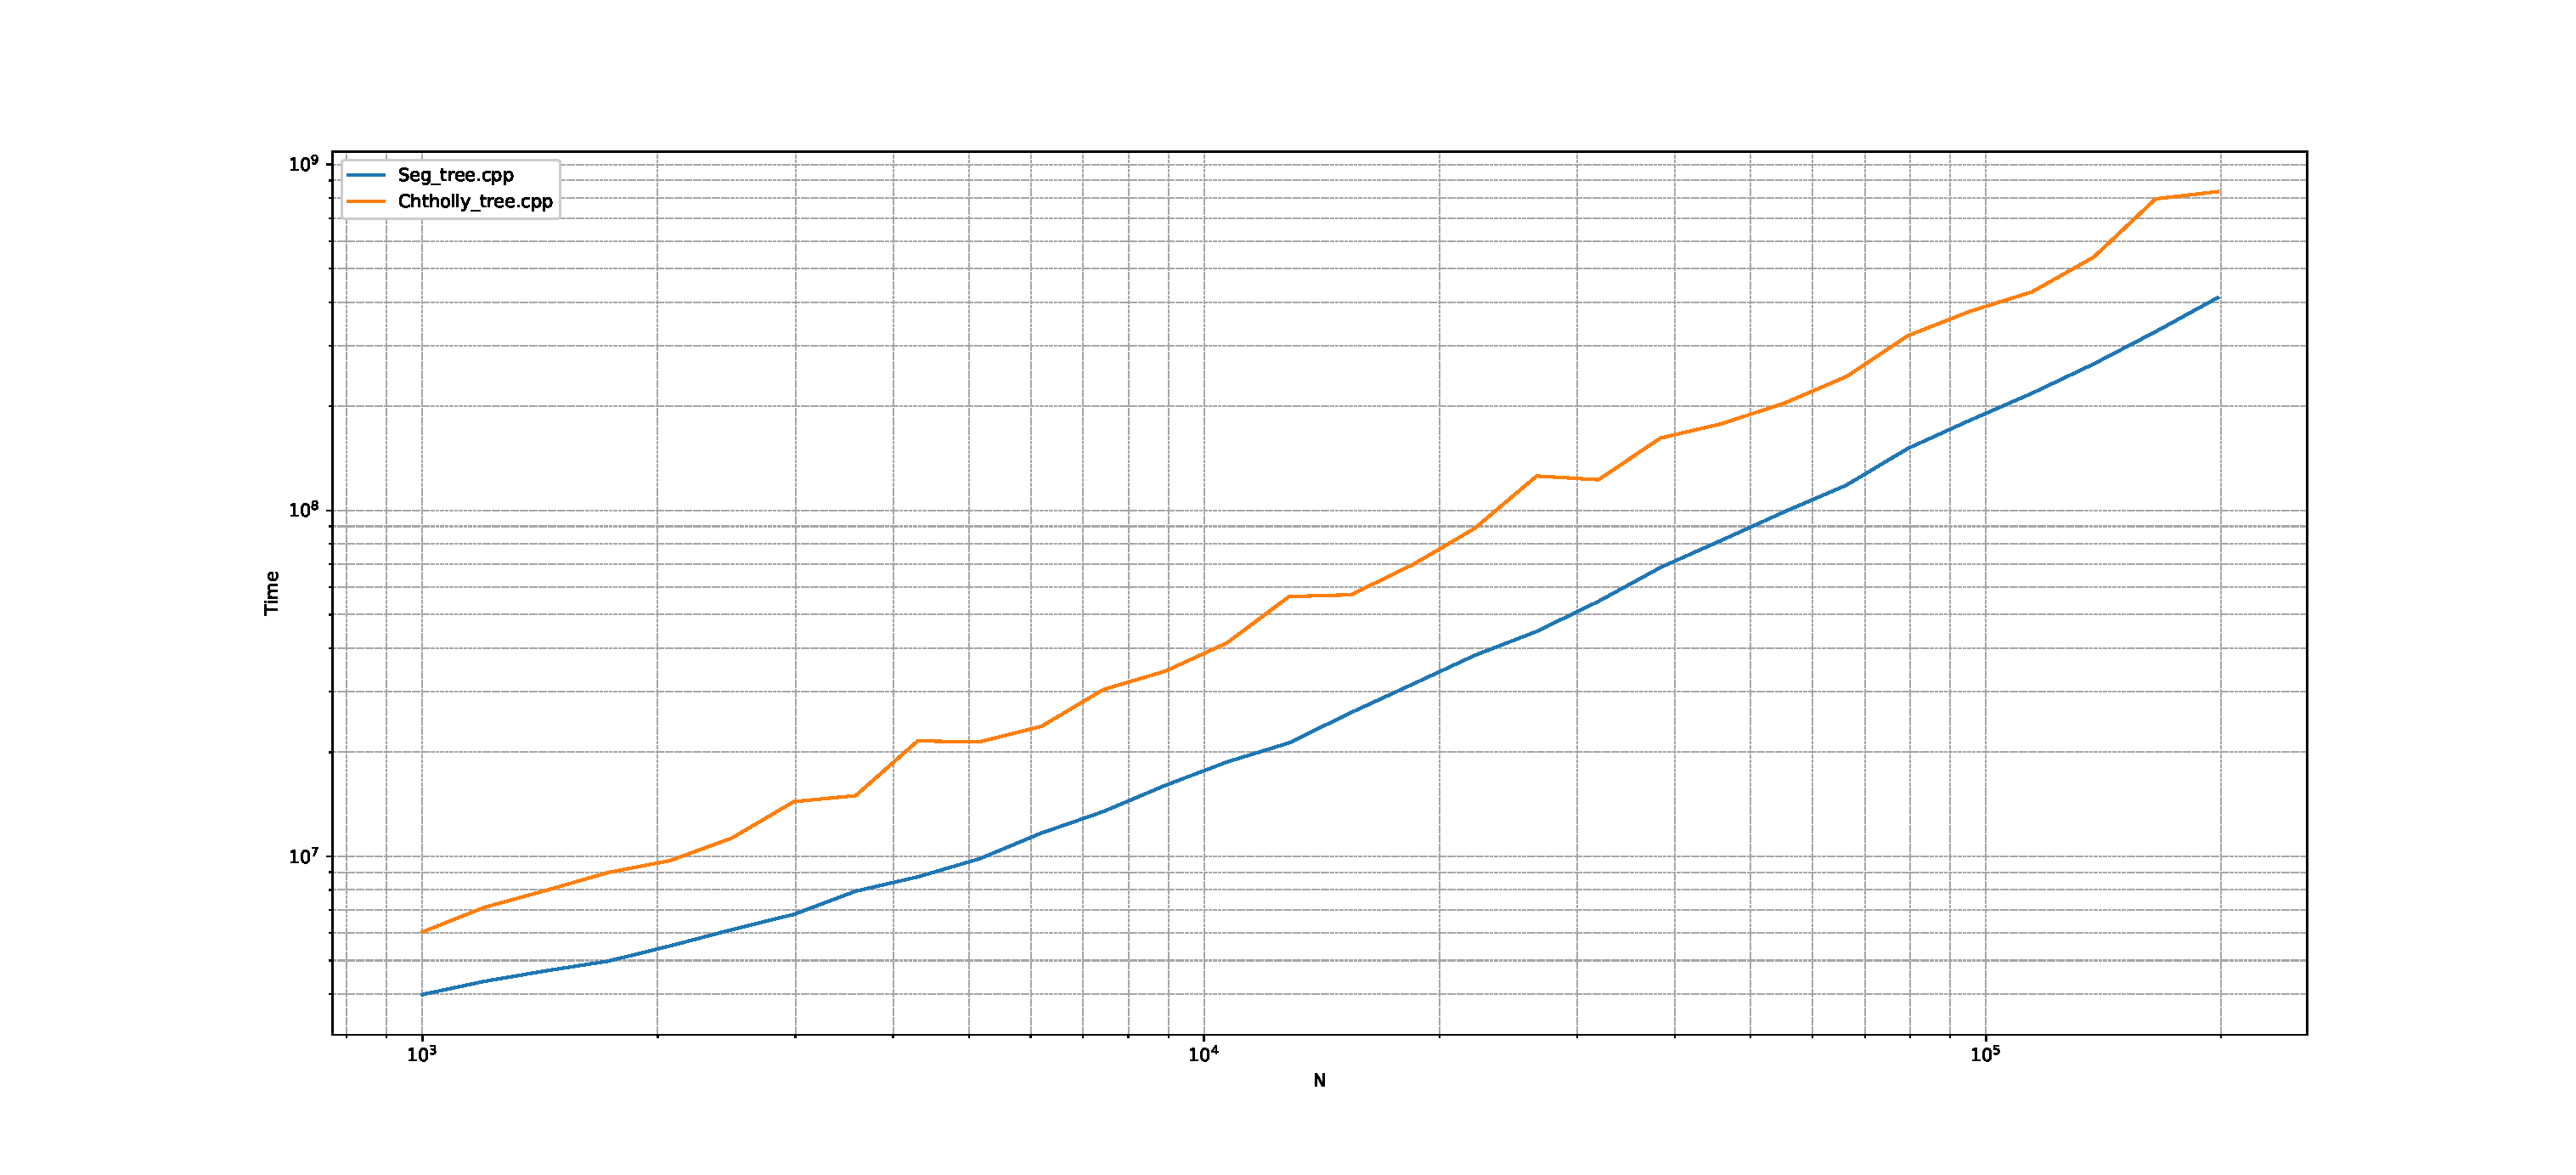
\includegraphics[width=\linewidth]{images/performance3.eps}
  \caption{混合任务下两数据结构的性能(双对数图,$M=N$)}
\end{figure}

不难发现,Chtholly树虽然实现简单,但在随机数据的情况下,与线段树差距不大。

\section{结论}

本文比较了各类支持区间操作的数据结构的实现方式,适用范围,局限性以及其时间、空间复杂度。此外,本文还利用实际数据,测量了在随机数据下一些支持区间操作的数据结构的性能,其结果与理论给出的结论相近。

从上面的比较不难看出,从通用性上看,朴素算法与Chtholly树是最佳的,其对区间操作的支持几乎没有限制;而Chtholly树的复杂度要远优于朴素算法,故值得使用。而从性能与通用性两者权衡的角度来看,线段树则是优先的选择。

如果仅考虑查询操作,则根据所查询的区间信息的性质,选取前缀和数组与ST表可以获得极好的性能;若要兼顾一些非密集的单点修改的操作,树状数组则是较好的权衡方案。

\section{讨论}

文中所提到的诸多数据结构,多数来自ACM界在实践中的创新,而很少见其发表于各类文献中。对于区间操作的需求,最初来自于计算机图形学:因为实际的空间中的物体的位置经常具有区间相互遮盖的关系。例如,线段树的提出,就是为了解决一类名为Klee's measure problem的图形学问题。此后,在计算机图形学迅猛发展期间,又出现了K-d Tree等由线段树发展而来的,维护高维区间的数据结构。

除了树状结构外,支持区间的操作的数据结构一般有以下几个思路:如果区间操作的性质良好,则考虑类似前缀等数学方式进行优化;如果区间操作的性质十分一般,则考虑使用分块的思想,而不对操作进行优化。总体上看,线段树既利用了分块的思想,又利用了区间操作的性质,故而其通用性和性能都十分均衡。如果区间操作的性质实在坏到极致,以至于无法用线段树实现,则Chtholly树和本文中没有提到的分块数据结构“莫队”,也较直接暴力求解有着很大的优势。

此外,面对一些新的需求,例如对区间的历史最值的查询等问题,其数据结构也是通过现有的数据结构改进而来,例如“可持久化线段树”等。又如在性能受限的平台上,由于线段树的实现复杂,其时间复杂度的常数较大,一种名为“Zkw线段树”的非递归线段树也相应地被提出。在理论界,对于传统的Range Minimum Query的研究也有较多成果,近年提出的很多算法甚至达到常数时间复杂度与线性空间复杂度,且近年的理论进展也逐步摸清了这类问题的复杂度下界。这些进展的背后除了突发的灵感外,有很多高观点的数学思想蕴含于其中。本文题目中因有“浅谈”二字,故不深入展开,仅作介绍而已,感兴趣的同学可以自行查阅学习。

实际的软件开发过程中,现有的成熟的数据库已经能够满足大部分的需求,但是在极端的需求下,这些精巧却少见的数据结构,对项目的性能,将会产生较大的作用。很多同学将这些支持奇怪操作的数据结构认为是奇技淫巧,但在笔者看来,或许并非如此。


\begin{acknowledgments}
  感谢讲授数据结构课程的张老师,和他的各位助教;没有他们的努力,就不会有如此优秀的课程。也感谢与笔者交流的同学们,他们的分享大大开阔了笔者的见识,使得笔者了解到课堂以外的一些有趣的数据结构。
\end{acknowledgments}


\nocite{*}

\bibliographystyle{cjc}
\bibliography{example}


\newpage

\appendix

\section{测评机环境}

\begin{lstlisting}[breaklines]
-------------------
OS: Linux x86_64
Kernel: 5.10.70-1-MANJARO
Uptime: 8 hours, 28 mins
Shell: bash 5.1.8
Resolution: 1536x864
Terminal: /dev/pts/0
CPU: Intel i3-10105 (8) @ 4.400GHz
GPU: Intel CometLake-S GT2 [UHD Graphics 630]
Memory: 867MiB / 15850MiB

GCC Version:
$ g++ -v
Using built-in specs.
COLLECT_GCC=g++
COLLECT_LTO_WRAPPER=/usr/lib/gcc/x86_64-pc-linux-gnu/11.1.0/lto-wrapper
Target: x86_64-pc-linux-gnu
Configured with: /build/gcc/src/gcc/configure --prefix=/usr --libdir=/usr/lib --libexecdir=/usr/lib --mandir=/usr/share/man --infodir=/usr/share/info --with-bugurl=https://bugs.archlinux.org/ --enable-languages=c,c++,ada,fortran,go,lto,objc,obj-c++,d --with-isl --with-linker-hash-style=gnu --with-system-zlib --enable-__cxa_atexit --enable-cet=auto --enable-checking=release --enable-clocale=gnu --enable-default-pie --enable-default-ssp --enable-gnu-indirect-function --enable-gnu-unique-object --enable-install-libiberty --enable-linker-build-id --enable-lto --enable-multilib --enable-plugin --enable-shared --enable-threads=posix --disable-libssp --disable-libstdcxx-pch --disable-libunwind-exceptions --disable-werror gdc_include_dir=/usr/include/dlang/gdc
Thread model: posix
Supported LTO compression algorithms: zlib zstd
gcc version 11.1.0 (GCC)

\end{lstlisting}






\end{document}
